
\documentclass[aps,pre,twocolumn,superscriptaddress]{revtex4-2}


\bibliographystyle{apsrev4-2}
\usepackage[colorlinks,linkcolor=blue,anchorcolor=blue,citecolor=blue,urlcolor=blue]{hyperref}


\usepackage{bm}
\usepackage{graphicx}
\usepackage{hyperref}
\usepackage{eucal}
\usepackage{amsmath}
\usepackage[capitalise]{cleveref}
\usepackage{wasysym}
\usepackage[toc,page]{appendix}


\begin{document}


\title{
Generation of plasma zonal flow shear by finite parallel wave length density fluctuations in slab geometry
}


\author{Y. Lang}
\author{Z.B. Guo}
\email[E-mail:]{zbguo@pku.edu.cn}
\affiliation{
School of Physics and State Key Lab of Nuclear Physics and Technology, 
Peking University, Beijing 100871, China
}

\date{\today}


\begin{abstract}
A possible zonal flow shear generation mechanism by drift wave turbulence in a cylindrical magnetized plasma with large relative density fluctuations is discussed. These fluctuations would introduce nonlinear terms in the vorticity equation other than the term related to Reynolds stress in Hasegawa-Wakatani equations. We show that a nonlinear term can explain the generation of zonal flow in a simulation of a linear magnetized plasma device. The simulated growth of zonal flow and profile of time-averaged Reynolds stress roughly agree with experimental observations. We thus show that in these experiments, when the relative density fluctuation is large, Reynolds force may not be the only mechanism for zonal flow generation.
\end{abstract}
\maketitle


\section{\label{sec:introduction}introduction}
The generation of zonal flow (ZF) in magnetically confined plasma is of wide interest, since it can impact the instabilities and turbulence and thus transport, especially at the edge of tokamaks \cite{Li_2020}. Through nonlinear interactions, energy can be transferred from drift waves (DW) to ZF \cite{Diamond_2005}. Whereas the mechanism of turbulent momentum transport, especially through the Reynolds stress term in the stress tensor, is extensively studied, other mechanisms can also be important in certain conditions \cite{Diamond_2009, Diamond_2013}.

For the study of ZF generation by collisional drift waves (CDW), the Controlled Shear Decorrelation Experiment (CSDX) with insulating endplates \cite{Thakur_2013} is a promising testbed, in that it is a simple drift wave-zonal flow system \cite{Xu_2010, Hajjar_2018} in uniform magnetic field and shares many similar scaling properties with tokamak boundaries \cite{Cui_2016}. Experiments on CSDX find nonlinear kinetic energy transfer from weak CDW turbulence to ZF \cite{Xu_2009, Xu_2010} and ZF driven by Reynolds force \cite{Holland_2006,Yan_2008,Yan_2010}. These works explains ZF generations in CSDX, with systematic sources of error, such as the neglect of electron temperature fluctuations in converting floating potential measured by Langmuir probes to plasma potential, which is used to calculate electric field and fluid velocity \cite{Holland_2006,Xu_2009}. Consequently, it can be helpful to do similar analysis in simulations.

Recently two 3D codes based on drift-reduced two-fluid cold-ion equations have focused on the simulations of CSDX $B=1000$ G insulating end-plates discharges \cite{Vaezi_2017V, Lang_2019} and compared to experimental observations. The code under BOUndary Turbulence (BOUT++) framework \cite{Vaezi_2017V} show considerable difference between actual (using plasma potential) and synthetic (using floating potential) Reynolds stress in the simulations, but do not quantitatively analyze the ZF generation in their simulations. In this paper, based on our flux-driven simulation \cite{Lang_2019}, we do detailed analysis on ZF generation in our simulated system.  

\section{\label{sec:theoretical model}theoretical model}
The system we are interested is a cylindrical plasma column in a uniform magnetic field $\bm{B}=B\hat{\bm{z}}$. The equilibrium of a given scalar field is its zonal average $\left<f\right>\equiv\int_{0}^{L_{\parallel}}\int_{0}^{2\pi}f \left(r,\theta,z\right)d\theta dz$ and its fluctuation is $\delta f\equiv f-\left<f\right>$, where $L_{\parallel}$ is the parallel wavelength of the DW and parallel periodicity is assumed. We use cold-ion and low-$\beta$ limit, so ion temperature and magnetic perturbations are neglected.
\subsection{\label{subsec:vorticity equation}vorticity equation}
The drift-reduce two-fluid vorticity equation comes from the continuity equations and quasi-neutrality, with the form of charge conservation \cite{Zeiler_1997}
\begin{equation}
	\nabla\cdot\left(n\bm{v}_{p}\right)+\nabla_{\parallel}j_{\parallel}=0~,
\label{eq:original vorticity}
\end{equation}
where 
\begin{equation}
	\bm{v}_{p}=-\frac{ec}{B\Omega_{i}}d_t\nabla_{\perp}\phi
\end{equation}
is the ion polarization drift. $\Omega_{i}\equiv eB/\left(m_{i}c\right)$ is the constant ion gyro-frequency. $d_{t}\equiv\partial_{t}+\bm{v}_{E}\cdot\nabla$ is the total time derivative. In this paper we adopt Boussinesq approximation \cite{Ricci_2012} to simplify the divergence of perpendicular current
\begin{equation}
	\nabla\cdot\left(nd_{t}\nabla_{\perp}\phi\right)\approx nd_{t}\nabla_{\perp}^{2}\phi~,
\label{eq:Boussinesq}
\end{equation}
which allows us to define vorticity by
\begin{equation}
	w\hat{\bm{z}}\equiv\nabla\times\bm{v}_{E}
	=\frac{c}{B}\nabla_{\perp}^{2}\phi\hat{\bm{z}}~.
\end{equation}
Discussions about gyro-fluid non-Boussinesq ZF generation can be found \cite{Held_2018}. The zonal average of vorticity equation \cref{eq:original vorticity} is then
\begin{equation}
\begin{aligned}
	\left<n\right>\partial_{t}\left<w\right>=&-\left<n\right>\left<\delta\bm{v}_{E}\cdot\nabla\delta w\right> \\
	&-\left<\delta n\left(\partial_{t}+\left<v_{E,\theta}\right>\frac{1}{r}\partial_{\theta}\right)\delta w\right> \\
	&+\left<\delta n\delta\bm{v}_{E}\cdot\nabla w\right>~.
\end{aligned}
\end{equation}
The first term on the right hand side (RHS) is the contribution of the divergence of vorticity flux, which is the perpendicular Reynolds force by the Taylor identity \cite{Li_2018,Diamond_1991}, to ZF
\begin{equation}
	-\left<\delta\bm{v}_{E}\cdot\nabla\delta w\right>
	=-\nabla\cdot\left<\delta\bm{v}_E\delta w\right>
	\approx\partial_r\left(-\partial_{r}\left<\delta v_{E,r}\delta v_{E,\theta}\right>\right)~,
\end{equation}
where in the last step we use the limit $\partial_{r}\gg 1/r$. This ZF generation mechanism has been extensively studied on CSDX \cite{Holland_2006,Yan_2008,Yan_2010,Thakur_2018} and is the only mechanism in Hasegawa-Wakatani (HW) systems \cite{Hasegawa_1983,Hajjar_2018}. The second term on the RHS can be neglected only when density fluctuations are small, i.e.
\begin{equation}
	\frac{\delta n}{\left<n\right>}\ll\frac{\omega_{nl}}{\omega},
\end{equation}
where $\omega_{nl}\equiv\delta\bm{v}_E\cdot\nabla$ is the nonlinear frequency and $\omega\equiv\partial_{t}+\left<v_{E,\theta}\right>\left(1/r\right)\partial_{\theta}$ is the DW frequency Doppler shifted by ZF. If this condition is not satisfied, we have to retain density fluctuation in the ion polarization current in \cref{eq:original vorticity}. Including ion-ion collisional viscosity $\mu_{\perp}$ and ion-neutral drag $\nu_{i,n}$ \cite{Vaezi_2017U}, the vorticity equation we use in our simulation \cite{Lang_2019} is
\begin{equation}
	\partial_{t}w=-\bm{v}_{E}\cdot\nabla w
	+\frac{\Omega_{i}}{e}\frac{1}{n}\nabla_{\parallel}j_{\parallel}
	+\mu_{\perp}\nabla_{\perp}^2 w+\mu_{\parallel}\nabla_{\parallel}^2w
	-\nu_{i,n}w~.
\label{eq:vorticity}
\end{equation}

\subsection{\label{subsec: ZF shear evolution}ZF shear evolution}
In this subsection we seek for the ZF driving mechanisms of ZF shear. Taking zonal average of \cref{eq:vorticity}, the left hand side (LHS) becomes
\begin{equation}
\begin{aligned}
	\left<\partial_{t}\nabla_{\perp}^{2}\phi\right>
&=\partial_{t}\left[\frac{1}{r}\partial_{r}
\left(r\left<v_{E,\theta}\right>\right)\right]\equiv S^{\dagger} \\
&\approx\partial_{t}\left(\partial_{r}\left<v_{E,\theta}\right>\right)\equiv S~.
\label{eq:S}
\end{aligned}
\end{equation}
In the second step we use the approximation $\partial_{r}\gg 1/r$, so this term becomes the evolution of zonal flow (ZF) shear. 

The first term on the RHS of \cref{eq:vorticity} becomes 
\begin{equation}
\begin{aligned}
	\left<-\bm{v}_{E}\cdot\nabla w\right>
	&=-\partial_{r}\left<v_{E,r}\frac{1}{r}\partial_{r}
	\left(rv_{E,\theta}\right)\right>\equiv F_{\perp}^{\dagger} \\
	&\approx-\partial_{rr}^{2}\left<v_{E,r}v_{E,\theta}\right>\equiv F_{\perp}~,
\label{eq:Fperp}
\end{aligned}
\end{equation}
where in the second step we use the approximation $\partial_{r}\gg 1/r$ for two times, and yield the radial derivative of Reynolds' force, which is able to drive ZF shear as we expected. 

Involving density fluctuations, the second term on the RHS of \cref{eq:vorticity} is nonlinear, and thus won't be canceled by zonal average, so it is also a possible drive of ZF shear. To study its physical meaning and properties, we decompose $j_{\parallel}$ using a electrostatic Ohm's law \cite{Zeiler_1997,Lang_2019}
\begin{equation}
j_{\parallel}=\frac{e}{\nu_{e}m_{e}}\left(\nabla_{\parallel}p_{e}-en\nabla_{\parallel}\phi\right)~.
\label{eq:Ohm}
\end{equation}
Large parallel heat conduction leads to $\nabla_{\parallel}T_{e}/T_{e}\ll\nabla_{\parallel}n/n$, so for \cref{eq:vorticity} we have
\begin{equation}
\begin{aligned}
	F_{\parallel}^{\dagger}
	&\equiv\frac{\Omega_{i}}{e}\left<\frac{1}{n}
	\nabla_{\parallel}j_{\parallel}\right> \\
	&\approx\frac{\Omega_{i}}{m_{e}}\left<\frac{1}{n}\nabla_{\parallel}
	\left[\frac{T_{e}}{\nu_{e}}\left(\nabla_{\parallel}n-en\frac{\nabla_{\parallel}
	\phi}{T_{e}}\right)\right]\right>~.
\label{eq:Fpar_dagger}
\end{aligned}
\end{equation}
Since $\delta n$ and $\delta T_{e}$ are usually in phase, the above approximation would result in a slight loss of total amplitude. In the lowest order of $F_{\parallel}^{\dagger}$, the remaining perturbations are $\nabla_{\parallel}\delta n$, $\nabla_{\parallel}\delta\phi$ and $\delta\left(1/n\right)$. Neglecting $\delta\left(T_{e}/\nu_{e}\right)$, we define an approximation of $F_{\parallel}^{\dagger}$ by
\begin{equation}
	F_{\parallel}\equiv\frac{\Omega_{i}}{m_{e}}\left<\frac{T_{e}}{\nu_{e}}\right>
	\left<\frac{1}{n}\nabla_{\parallel}
	\left(\nabla_{\parallel}n-en\frac{\nabla_{\parallel}
	\phi}{T_{e}}\right)\right>~.
\label{eq:Fpar}
\end{equation}
For density and potential perturbations of collisional drift wave (CDW) in linear devices, the amplitude $\left|e\delta\phi/T_{e}\right|/\left|\delta n/n\right|\apprle 1$ and the cross-phase $\xi\left(\delta n,\delta\phi\right)<\pi/4$ \cite{Thakur_2014,Jassby_1972}. Therefore, for weakly non-adiabatic electrons as in CSDX \cite{Hong_2018G,Hong_2018T}, one would expect a secondary change of $F_{\parallel}$ if $\nabla_{\parallel}\phi$ is neglected
\begin{equation}
	F_{\parallel}\approx G_{\parallel}
	\equiv \frac{\Omega_{i}}{m_{e}}\left<\frac{T_{e}}{\nu_{e}}\right>
	\left<\left(\frac{\nabla_{\parallel}n}{n}\right)^{2}\right>~.
\label{eq:Gpar}
\end{equation}
\cref{eq:Gpar} shows that, the main part of $F_{\parallel}^{\dagger}$, $G_{\parallel}$, is positive definite. Consequently, at the edge of tokamaks, non-adiabatic electrons should always introduce a finite drive of positive $E_{r}$ shear.
The full zonal-average of \cref{eq:vorticity} is then
\begin{equation}
	\partial_t S^{\dagger}=F_{\perp}^{\dagger}+F_{\parallel}^{\dagger}+
	D_{\perp}\frac{1}{r}\frac{\partial}{\partial r}
	\left(r\frac{\partial}{\partial_{r}}S^{\dagger}\right)-
	\gamma S^{\dagger}~.
\end{equation}


\section{\label{simulation setup} simulation setup}
As has been clarified in the erratum \cite{Lang_2020} of our previous paper \cite{Lang_2019}, the expression of classical diffusion coefficient we used has a minor mistake. In this paper we fix this by setting
\begin{equation}
\begin{aligned}
	D_{\perp}&=\chi_{\perp} \\
	&=1.652\times 10^5\frac{0.5n_0}{\mathrm{cm^{-3}}}
	\left(\frac{0.5T_{0}}{\mathrm{eV}}\right)^{-1/2}
	\left(\frac{B}{\mathrm{G}}\right)^{-2}\ln\Lambda_{0}\mathrm{cm^2/s}~,
\end{aligned}
\end{equation}
where $n_0=1\times 10^{13}\ \mathrm{cm^{-3}}$ and $T_0=3\ \mathrm{eV}$ are peak density and electron temperature in the shear flow growth phase and used for the normalization, so $0.5n_0$ and $0.5T_0$ are approximately equilibrium density and temperature at peak gradient and thus peak CDW amplitude position, $r\simeq3$ cm, where we are especially interested. The ion-ion viscosity $\mu_{\perp}$ is also altered to $4.8\times10^3\ \mathrm{cm^2/s}$ to match the parameters at $r\simeq 3$ cm \cite{Vaezi_2017U}. For now, all diffusion coefficients we use in the simulation are constants, estimated using experimentally diagnosed parameters near $r=3$ cm, which simplifies the physics and simulation difficulty, but may introduce some disagreement with experiments. Except for this and an increased spacial resolution, $nx=ny=22$, $nz=22$, we use exactly the same simulation setup as in \cite{Lang_2019}. Here we repeat the equations
\begin{equation}
d_{t}T_{e}
=-\frac{2}{3}T_{e}\nabla_{\parallel}v_{\parallel e}
+\chi_{\perp}\nabla_{\perp}^{2}T_{e}+\chi_{\parallel}\nabla_{\parallel}^{2}T_{e}
-\gamma T_{e}+S_{T_{e}}~,
\label{Te}
\end{equation}
\begin{equation}
d_{t}n
=-\nabla_{\parallel}\left(nv_{\parallel e}\right)
+D_{\perp}\nabla_{\perp}^{2}n+D_{\parallel}\nabla_{\parallel}^{2}n
-\gamma n+S_{n}~,
\label{den}
\end{equation}
\begin{equation}
d_{t}v_{\parallel i}
=-\frac{T_{e}}{n}\nabla_{\parallel}n
+\mu_{\perp}\nabla_{\perp}^{2}v_{\parallel i}
+\mu_{\parallel}\nabla_{\parallel}^{2}v_{\parallel i}
-\nu_{i,n} v_{\parallel i}~,
\label{vi}
\end{equation}
\begin{equation}
d_{t}w
=\frac{\Omega_i}{e}\frac{1}{n}\nabla_{\parallel}j_{\parallel}
+\mu_{\perp}\nabla_{\perp}^{2}w+\mu_{\parallel}\nabla_{\parallel}^{2}w
-\nu_{i,n} w~,
\label{w}
\end{equation}
where $S_{T_e}$ and $S_n$ are artificial temperature and density sources to make our flux-driven simulation produce profiles that are roughly close to CSDX experiment \cite{Tynan_2009} before its upgrade in 2014 \cite{Thakur_2014} .

We briefly summarize the results in \cite{Lang_2019} that are relevant to (and also reproduced in) this paper. Qualitatively, the turbulence character undergoes a periodic evolution, which is an example of the scenario described in section 3.4.1 of \cite{Diamond_2005}. Each period is separated into two phases. The first phase is called shear flow growth phase, which is characterized by the growth of the primary instability, i.e. $m\simeq3$ DW, whose secondary instability produces $m=0$ ZF, where $m$ is the azimuthal mode number. The second phase is called collapse phase, begins with the onset of $m\simeq1$ Kelvin-Helmholtz instability (KHI), which is triggered by both ZF and CDW. Recombination and helicon source then bring the plasma back to shear flow growth phase.

\section{\label{sec:shear flow growth phase}shear flow growth phase}
The shear flow growth phases in the simulation share the same physics. In this section we focus on one of them for detailed analysis.

A typical shear flow growth phase of CSDX is shown in \Cref{fig:acc_den_drive}, revealing that our approximations in \Cref{eq:Fpar_dagger,eq:Fpar,eq:Gpar} are basically valid, especially for $r<3$ cm, where perturbations are much smaller than the corresponding zonal component.
\begin{figure}[htb]
	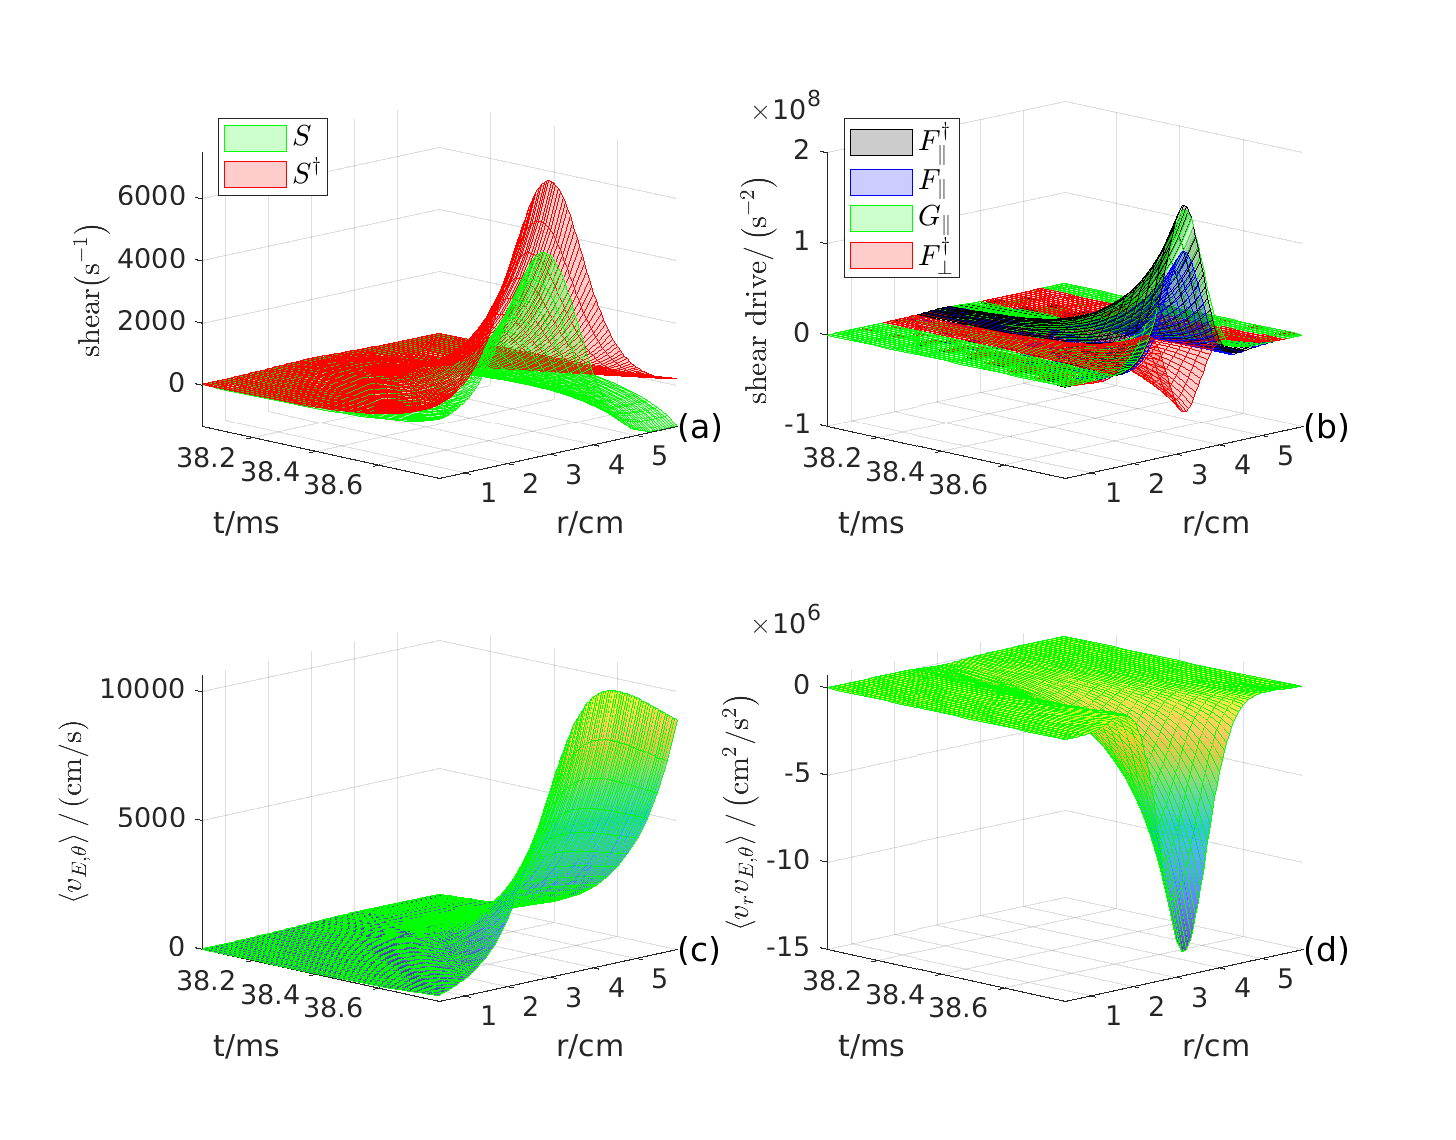
\includegraphics[width=3.375 in]{acc_den_drive.eps}
	\caption{
		Simulation result of some zonal-averaged fields in a typical shear flow growth phase. (a) evolution of flow shear, defined in \Cref{eq:S}. (b) evolution of flow shear drives, defined in \Cref{eq:Fperp,eq:Fpar_dagger,eq:Fpar,eq:Gpar}.
		\label{fig:acc_den_drive}	
	}
\end{figure}


As can be seen in \Cref{fig:acc_den_drive}(a), the flow shear grows globally, with the maximum amplitude near $r\approx 3$ cm, where $\left<n\right>$ and $\left<T_{e}\right>$ has the maximum gradient, and the instability has the maximum intensity. \Cref{fig:acc_den_drive}(b) shows that, the main drive of zonal flow shear is $F_{\parallel}^{\dagger}$, and $F_{\perp}^{\dagger}$flattens the flow profile. The resulting growth of $\bm{E}\times\bm{B}$ is shown in \Cref{fig:acc_den_drive}(c), which can be compared to time-delay estimation (TDE) results in \cite{PhysRevLett.104.065002,doi:10.1063/1.3322823}. Note that the TDE result would include CDW phase velocity as explained in \cite{PhysRevE.100.033212}. Reynolds' stress can be regarded as ZF flux, peaking near the maximum ZF shear location (\Cref{fig:acc_den_drive}(d)), convecting ZF down its gradient. 


As a validation of our simulation, we compare our simulation result of Reynolds' stress with experimental observations. For the argon plasma in CSDX, the sheath potential coefficient in \Cref{eq:phif} is estimated by \cite{Nie_2018}
\begin{equation}
	\Lambda=\frac{1}{2}\ln\left(\frac{m_{i}}{2\pi m_{e}}\right)\approx 4.68~,
\label{eq:Lamda}
\end{equation}
which is significantly larger than deuterium plasmas, making the approximation $\phi\approx\phi_{f}$ easier to break down. The breaking in our simulation is shown in \Cref{fig:comp_pl_fl}. In spite of a somewhat unknown filter used in experiments, our simulation results of time-averaged synthetic $\left<v_{E,r}v_{E,\theta}\right>$ and $\left<v_{E,r}^{2}\right>$ agree with experimental observations well \cite{doi:10.1063/1.2985836,PhysRevLett.104.065002}. However, when we use plasma potential $\phi$, the amplitude of the two profiles reduce significantly, and the Reynolds' stress changes shape.

\begin{figure}[htb]
	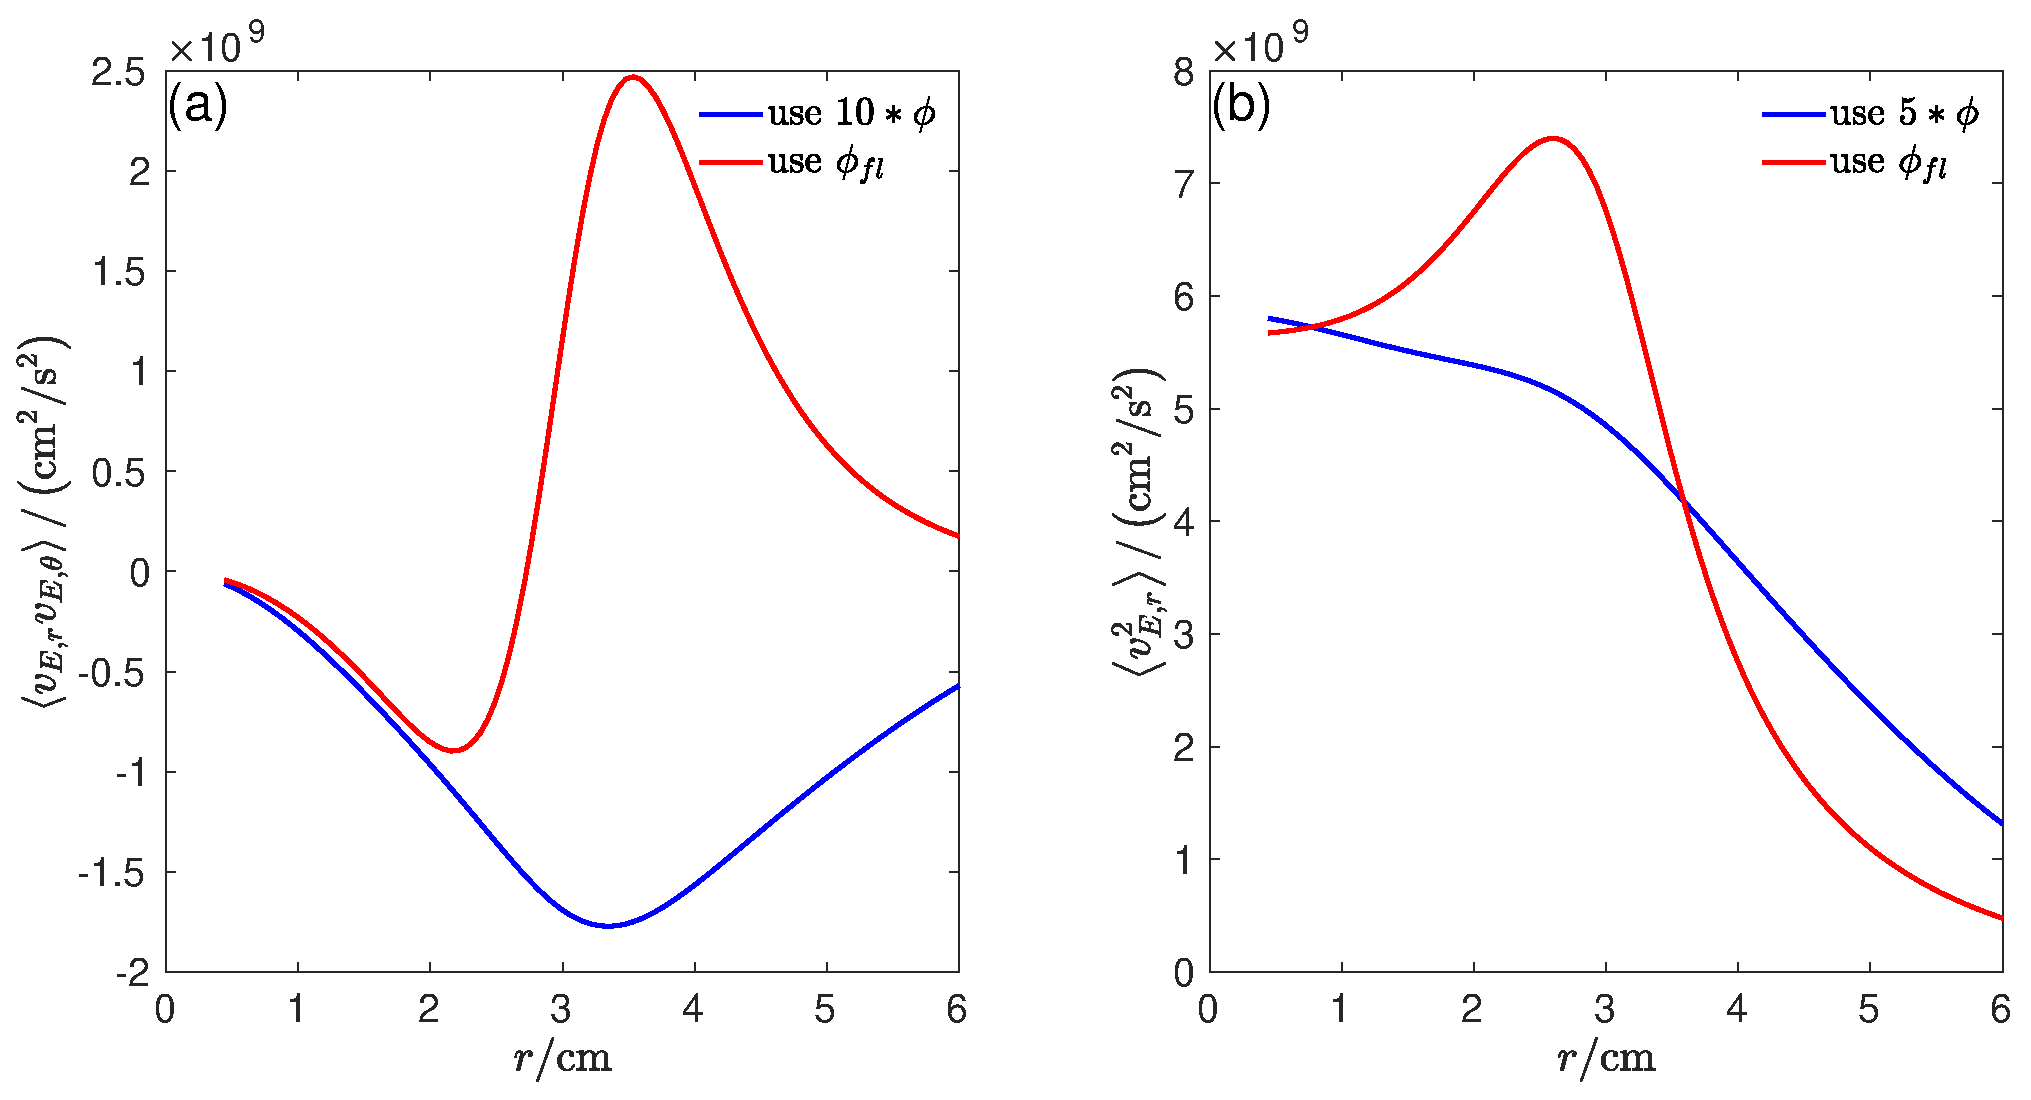
\includegraphics[width=3.375 in]{comp_pl_fl.eps}
	\caption{
		Simulation result of some zonal and time averaged fields during $t=9.4-50.8$ ms. The blue curves are calculated using multiples of plasma potential, while the red curves are calculated using synthetic floating potential given by \Cref{eq:phif,eq:Lamda}. (a) Reynolds' stress and (b) the intensity of radial $\bm{E}\times\bm{B}$ velocity perturbations.
		\label{fig:comp_pl_fl}	
	}
\end{figure}


\bibliography{ZF.bib}



\end{document}

